\documentclass[11pt]{article}
%
\usepackage[hyperref,dvipsnames]{xcolor}
\usepackage{hyperref}
\definecolor{darkblue}{rgb}{0,0,.5}                                                                                                 
\definecolor{black}{rgb}{0,0,0}                                                  
                                                                                 
\hypersetup{                                                                     
	breaklinks=true,                                                             
	bookmarksnumbered=true,                                                      
	bookmarksopen=true,                                                          
	bookmarksopenlevel=1,                                                        
	breaklinks=true,                                                             
	colorlinks=true,                                                             
	pdfstartview=Fit,                                                            
	pdfpagelayout=SinglePage,                                                    
	%                                                                            
	filecolor=darkblue,                                                          
	urlcolor=darkblue,                                                           
	linkcolor=black,                                                             
	citecolor=black                                                              
}

\usepackage{geometry}
\geometry{a4paper}
\usepackage{amssymb}
\usepackage{amsmath}
\usepackage{amsthm}
\usepackage[no-math]{fontspec}
\defaultfontfeatures{Mapping=tex-text}
\usepackage{polyglossia}
\setmainlanguage[spelling=new,babelshorthands=true]{german}
\usepackage{xltxtra}
\usepackage{graphicx}
\usepackage{float}
\usepackage{floatflt}
\usepackage{icomma}
%\usepackage{comment}
\usepackage{caption}
\usepackage{enumerate}
\usepackage{array}
\usepackage{tabularx}
\usepackage{cleveref}
\usepackage{accents}

\newcommand{\ubar}[1]{\underaccent{\bar}{#1}}
%
%\newcommand{\eq}[1]{\begin{align*}#1\end{align*}}
%\newcommand{\eqt}[1]{\begin{align}#1\end{align}}
%\newcommand{\mat}[1]{\left (\begin{matrix}#1\end{matrix}\right )}
\newcommand{\pd}[1]{\frac{\partial}{\partial {#1}}}
%%\newcommand{\qed}{\begin{flushright}$\square$\end{flushright}}
%\newcommand{\qed}{\hfill $\square$}
\newcommand{\dotp}[2]{\langle #1, #2 \rangle}
\newcommand{\pdot}{\,\cdot\,}
\newcommand{\norm}[1]{\|#1\|}
%\newcommand{\mrm}[1]{\mathrm{#1}}
%\newcommand{\satz}[2]{\paragraph{Satz #1:}#2}
%\newcommand{\bew}[1]{\paragraph{Beweis:}#1}
%\newcommand{\defn}[2]{\paragraph{Definition #1:}#2}
%\newcommand{\bsp}[1]{\paragraph{Beispiel:}#1}
%\newcommand{\bem}[1]{\paragraph{Bemerkung:}#1}
%\newcommand{\kor}[2]{\paragraph{Korollar #1:}#2}
%\newcommand{\lemma}[2]{\paragraph{Lemma #1:}#2}
\renewcommand{\O}{\mathcal O}
%\newcolumntype{M}{>{$}c<{$}}
%%\renewcommand*\arraystretch{1.5}
%\newcommand{\C}{\operatorname{C}}
%\renewcommand{\epsilon}{\varepsilon}
\renewcommand{\phi}{\varphi}
%\renewcommand{\Re}{\operatorname{Re}}
%\renewcommand{\Im}{\operatorname{Im}}
%\renewcommand{\d}{\; \mathrm{d}}
\newcommand{\D}{\mathrm{D}}
%\newcommand{\supp}{\operatorname{supp}}
%\newcommand{\diag}{\operatorname{diag}}
%\newcommand{\Bild}{\operatorname{Bild}}
%\newcommand{\Span}{\operatorname{Span}}
%\newcommand{\Kern}{\operatorname{Kern}}
%\newcommand{\pdef}[1]{\left\{\begin{array}{lc}#1\end{array}\right.}
\newcommand{\R}{\mathbb{R}}
\newcommand{\N}{\mathbb{N}}
\newcommand{\p}{\mathcal{P}}
\newcommand{\LM}{\mathcal{M}}
\newcommand{\op}{\operatorname}
\newcommand{\prob}[1][\mu]{\big(P(#1)\big)}
\newcommand{\rprob}[1][\mu]{\big(P_N(#1)\big)}
\newcommand{\set}[1]{\left\{#1\right\}}
\newcommand{\spn}{\operatorname{span}}
\newcommand{\seq}[1]{\left(#1\right)}
\newcommand{\dist}{\operatorname{dist}}

\newcommand{\beginwithlist}{\leavevmode \vspace{-\baselineskip}}
\newcommand{\beginwithlistbem}{\leavevmode}
\newcommand{\beginwithlistbew}{\leavevmode}

\numberwithin{equation}{section}
\renewcommand{\labelenumi}{\roman{enumi}\,)}

\newtheoremstyle{mythmstyle}
	{\baselineskip}%		space above
	{\baselineskip}%		space below
	{}%			body font
	{}%			indent
	{\bfseries}%			head font
	{}%			punctuation after head
	{\newline}%	space after head
	{}%			'theorem head spec'

\theoremstyle{mythmstyle}

\newtheorem{satz}{Satz}[section]
\newtheorem{defn}[satz]{Definition}
\newtheorem{lemma}[satz]{Lemma}
\newtheorem{kor}[satz]{Korollar}
\newtheorem{bsp}[satz]{Beispiel}

\theoremstyle{definition}

\newtheorem*{bem}{Bemerkung}

\usepackage{mathtools}
\usepackage{pgfplots}

\begin{document}

\begin{center}
	Vorlesungsmitschrift\\
	\huge \textsc{Reduzierte Basis Methoden}\\[0.5cm]
	\large \textsc{Universität Stuttgart, SS15}\\
	Prof. Dr. Bernard Haasdonk\\[0.2cm]
\end{center}

\vspace{\baselineskip}

\begin{tabularx}{0.9\textwidth}{Xl}
	\small \textsc{Autoren}: & \textsc{Stand}:\\
	Stefan Simeonov & \today 
\end{tabularx}

\vspace{2\baselineskip}

\tableofcontents

\pagebreak

\section{Einleitung}
\label{sec-1}

\subsubsection*{Parameterabhängige Probleme}
\label{Parameterabhängige Probleme}

\begin{bsp}[Parameterabhängige PDE]
	Sie $\Omega \subseteq \R^d$ polygonales Gebiet. Zu Parametervektor $\mu \in \mathcal{P} \subset \R^p$ aus einer Menge $\mathcal{P}$ von "`erlaubten"' Parametern ist eine Funktion (z.\,B. "`Temperatur"') $u(\mu): \Omega \rightarrow \R$, s.\,d.:
	\begin{align*}
		\nabla \cdot (\kappa(\mu) \nabla u) &= q(\mu) & \text{in } \Omega \\
		u(\mu) &= 0 & \text{auf } \delta\Omega
	\end{align*}
	mit $\kappa(\mu) : \Omega \rightarrow \R$ (z.\,B. "`Wärmeleitungskoeffizient"') \\
	und $q(\mu) : \Omega \rightarrow \R$ (z.\,B. "`Wärmequelle/-senke"') \\
	
	z.\,B. $q(x;\mu) := \begin{cases}
			1 & \text{für } x \in \Omega_q \\
			0 & \text{sonst}
		\end{cases}$
\\

Weiter kann Ausgabe erwünscht, z.\,B. mittlere Temperatur
	\[
		s(\mu) = \frac{1}{|\Omega_s|} \int u(x; \mu) \,dx
	\]
	
\begin{figure}[H]
  \centering\small
    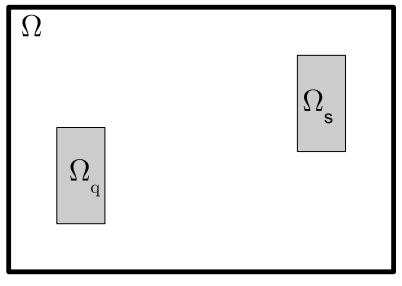
\includegraphics[width = 0.5 \textwidth]{Bilder/MittlereTemp.png}
  \caption{Beispiel Wärmeleitung mit Quelle $\Omega_q$ und Messbereich $\Omega_s$}{(aus B. Haasdonk, Reduzierte-Basis-Methoden, Skript zur Vorlesung SS 2011, Universität Stuttgart, IANS-Report 4/11, 2011.)}
  \label{fig:MittlereTemp}
\end{figure}
\end{bsp}

\begin{bsp}[Parametrisches stationäres System]
Zu Parameter $\mu \in \mathcal{P} \subseteq \R^p$ ist Zustandsvektor $u(\mu) \in \R^n$ und Ausgabe $s(\mu) \in \R^k$ gesucht, s.\,d.:
\begin{align*}
	0 &= A(\mu) \cdot u(\mu) + B(\mu) w(\mu) \\
	s(\mu) &= l(\mu) \cdot u(\mu)
\end{align*} 
mit parameterabhängigen Matrizen $A(\mu) \in \R^{n\times n}, B(\mu) \in \R^{n\times m}, C(\mu) \in \R^{k \times n}$ mit Eingabevektor $w \in \R^m$.
\end{bsp}

\subsubsection*{Schwache Formulierung in Hilberträumen}
\label{Schwache Formulierung in Hilberträumen}

Sie $X$ reeller Hilbertraum (reel, seperabel). Zu $\mu \in \mathcal{P}$ ist gesucht ein $u(\mu) \in X$ und $s(\mu) \in \R$
\begin{align*}
	a(u(\mu),v; \mu) &= f(v; \mu) \\
	s(\mu) &= l(u(\mu); \mu) & \forall v \in X
\end{align*}
Mit Bilinearform $a(\pdot,\pdot; \mu)$ und Linearform $f(\pdot; \mu)$, $l(\pdot; \mu)$. Beide Beispiele lassen sich so formulieren.

z.\,B. 1.1: 
\begin{align*}
	X=H_0^1(\Omega):=\{f\in L^2(\Omega) | \pd{x_i}& f \in L^2(\Omega), f_{|\delta\Omega} = 0\} \\
	\underbrace{\int_{\Omega} \kappa (x; \mu) \nabla u(x; \mu) \cdot \nabla v(x) dx}_{a(u(\mu),v; \mu)} &= \underbrace{\int_{\Omega} q(x; \mu) \cdot v(x) dx}_{f(v; \mu)} &\forall v \in X \\
	s(\mu) = \frac{1}{|\Omega_s|} \int_{\Omega_s} u(x; \mu) &=: l(u(\mu); \mu)
\end{align*}

Zu Bsp. 1.2 ($k=1$, "`single output"') \qquad $X = \R^n$
\begin{align*}
	\underbrace{v^TA(\mu)u(\mu)}_{a(u(\mu),v; \mu)} &= \underbrace{-v^TBw}_{f(v; \mu)} \\
	s(\mu) &:= \underbrace{C(\mu)u(\mu)}_{l(u(\mu); \mu)}
\end{align*}

In der Vorlesung werden weitere Verallgemeinerungen zu $a:X_1 \times X_2 \rightarrow \R$ mit $X_1 \neq X_2$, nichtlinear und instationäre Probleme behandelt.

\subsection{Modellreduktion}
\label{Modellreduktion}

\subsubsection*{Grundidee/Motivation}
\label{Grundidee/Motivation}

\begin{itemize}
	\item $\mathcal{M}:= \{u(\mu) | \mu \in \mathcal{P}\} \subset X$ für $\mathcal{P} \subseteq \R^p$ ist die durch $\mu$ parametrisierte Lösungsmannigfaltigkeit.
	\item $X$ ist im allgemeinen $\infty$-dimensional Sobolev-Raum) oder endlich- aber  sehr hochdimensional (FEM, FV, FD-Raum). $\mathcal{M}$ ist aber höchstens $p$-dimensional. \\
	$\Rightarrow$ Motivation für Suche nach einem niedrigdimensionalen Teilraum $X_n \subseteq X$ zur Approximation von $\mathcal{M}$ und einer Approximation $u_N(\mu) \approx u(\mu), u_N(\mu) \in X_N$
	\item Insbesondere bei Reduzierten-Basis-Methoden (RB-Methoden): \\
	$X_N$ durch Beispiellösungen erzeugt, sog. "`Snapshots"' \\
	$X_N \subseteq \op{span}\{u(\mu_1),...,u(\mu_n)\}$ für geeignete Parameterwerte $\mu_i \in \mathcal{P}$. \\
	Ziel ist außerdem Fehlerkontrolle durch Schranken $\Delta_N(\mu)$: \\
	\[
	||u(\mu) - u_N(\mu)|| \le \Delta_N(\mu)
	\]
\end{itemize}

\subsubsection*{Illustration}

\begin{figure}[H]
  \centering\small
    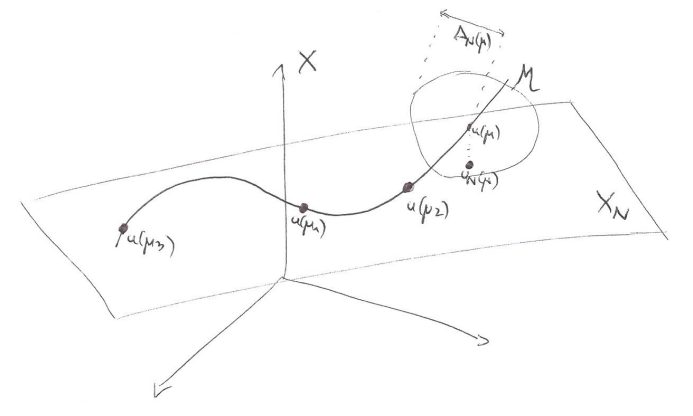
\includegraphics[width = 0.7 \textwidth]{Bilder/IllustrationM.png}
  \caption{Parametrisierte niedrigdimensionale Lösungsmenge}{(aus dem Online-Skript von Prof. Dr. Haasdonk zu Reduzierte Basen 2015)}
  \label{fig:IllustrationM}
\end{figure}

\begin{bsp}
	Gesucht ist $u(\mu) \in C^2([0,1])$ mit 
	\begin{align*}
		(1 + \mu) u'' &= 1 & \text{auf} (0,1) \\
		u(0) &= u(1) = 1
	\end{align*}
	Für $\mu \in [0,1] =: \mathcal{P} \subseteq \R$. Spezielle Lösungen ("`Snapshots"')
	\begin{align*}
		\mu &= 0 \Rightarrow u_0(x) = u(x; \mu = 0) = \frac{1}{2} x² - \frac{1}{2} x + 1 \\
		\mu &= 1 \Rightarrow u_1(x) = u(x; \mu = 1) = \frac{1}{4} x² - \frac{1}{4} x + 1 \\
	\end{align*}
	RB-Raum: $X_N := \op{span}(u_0,u_1)$
	Reduzierte Lösung gegeben durch
	\begin{align*}
		u_N(\mu) &:= \alpha_0(\mu)u_0 + \alpha_1(\mu)u_1 \\
		\alpha_0 (\mu) &= \frac{2}{\mu + 1} - 1 ; \qquad \alpha_1(\mu) = 2 - \frac{2}{\mu + 1}
	\end{align*}
	Diese erfüllt 
	\[
	 ||u_N(\mu) - u(\mu)||_{\infty} = \sup\limits_{\mu} ||u(\mu) - u_N(\mu)|| = 0
	\]
	ist somit exakt. $\mathcal{M}$ ist enthalten in 2-dimensionalem Unterraum $X_N$: Genauer $\alpha_0 + \alpha_1 = 1,\, 0 \le \alpha_0,\, \alpha_1 \le 1$, also ist $\mathcal{M}$ Menge der Konvexkombinationen von $u_0$, $u_1$.
\end{bsp}

\subsubsection*{Begriffe}
\label{Begriffe}

\begin{itemize}
	\item Eine PDE ist ein \emph{analytisches} Modell, welches die \emph{exakte Lösung} $u(\mu) \in X$ in einem typischerweise $\infty$-dimensionalen Funktionenraum $X$ charakterisiert.
	\item Ein \emph{detailliertes Modell} (auch \emph{hochdimensionales Modell}) ist ein Berechnungsverfahren oder charakterisiert eine Approximation $u(\mu) \in X$ in hochdimensionalen Raum mit sehr allgemeinen Approximationseigenschaften. (z.\,B. FEM/FV/FD, dim $X = 10^3 - 10^8$).
	In dieser Vorlesung kann $u(\mu)$ sowohl eine analytische als auch eine detaillierte Lösung darstellen.
	\item Ein \emph{reduziertes} Modell ist ein Berechnungsverfahren bzw. eine Charakterisierung einer reduzierten Lösung $u_N(\,u)$ in einem sehr problemangepassten Raum $X_N$ (dim $X_N = 1 - 10^3$).
	\item \emph{Modellreduktion} beschäftigt sich mit Methoden der Erzeugung reduzierter Modelle und Untersuchung ihrer Eigenschaften
	\item Modellreduktion ist ein modernes Gebiet der angewandten Mathematik und Ingenieurwissenschaften (Schwerpunkt in SimTech PN3, MOR-Seminar)
\end{itemize}

\subsubsection*{Anwendungen für parametrische reduzierte Modelle}
\label{Anwendungen für parameterische reduzierte Modelle}

"`Kleinere"' Modelle stellen geringere Anforderungen an Rechenzeit und Speicher, daher Einsatz in:

\begin{itemize}
	\item "`multi-query"'-Kontext, d.\,h. Vielfachanfragen unter Parametervariation: Parameterstudien, Design, Parameteridentifikation, Inverse Probleme, Optimierung, statistische Analyse
	\item Multi-skalen-Modelle (reduzierte Mikrolöser)
	\item "`real-time"'-Kontext, d.\,h. Anwendungen mit schneller Simulationsantwort: Interaktive Benutzeroberfläche, Web-Formulare, Echtzeitsteuerung von Prozessen
	\item "`cool-computing"'-Kontext, d.\,h. Simulation auf "`einfacher"' Hardware: elektronische Regler, Smartphones, Ubiquitious Computing
\end{itemize}

\subsubsection*{Demonstration}
\label{Demonstration}

\textsf{demo\_thermalblock.m} aus \textsf{RBmatlab}, Smartphone App JaRMoS

\begin{figure}[H]
  \centering\small
    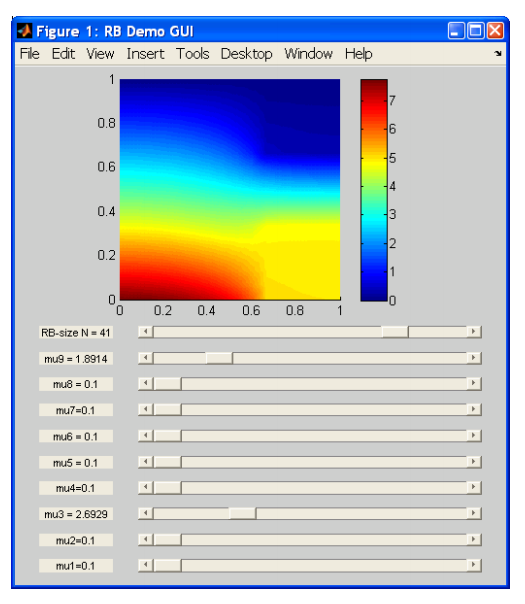
\includegraphics[width = 0.7 \textwidth]{Bilder/ThermoBlock.png}
  \caption{Beispiel des Thermischen Blocks aus \textsf{demo\_thermalblock.m}}{(aus B. Haasdonk, Reduzierte-Basis-Methoden, Skript zur Vorlesung SS 2011, Universität Stuttgart, IANS-Report 4/11, 2011.)}
  \label{fig:ThermoBlock}
\end{figure}

\subsubsection*{Offline/Online Zerlegung}
\label{Offline/Online Zerlegung}

Typischerweise wird eine Verechnungsintensive Generierung des reduzierten Modells akzeptiert, sog. \emph{Offline-Phase}. Dies ermöglicht schnelle Anwendbarkeit des reduzierten Modells in der \emph{Online-Phase}. Offline-Kosten werden gerechtfertigt durch Amortisierung im multi-query-Kontext, d.\,h. Laufzeitgewinn bei genügend großer Anzahl an Online-Simulationen

\begin{figure}[H]
  \centering\small
    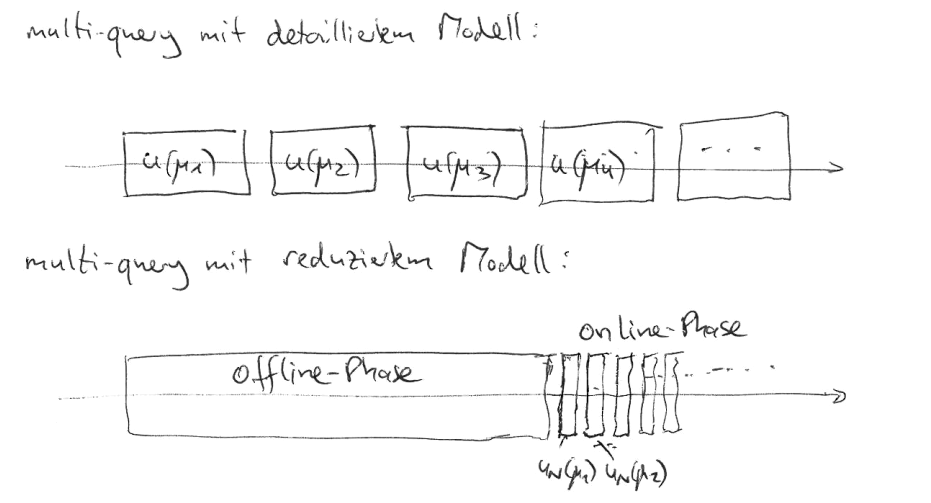
\includegraphics[width = 0.6 \textwidth]{Bilder/OfflineOnline.png}
  \caption{Laufzeitvergleich eines detaillierten mit einem reduzierten Modell}{(aus dem Online-Skript von Prof. Dr. Haasdonk zu Reduzierte Basen 2015)}
  \label{fig:OfflineOnline}
\end{figure}

\subsubsection*{Zentrale Fragen}
\label{Zentrale Fragen}

\begin{itemize}
	\item Reduzierte Basis: Wie kann ein möglichst kompakter Teilraum konstruiert werden? Können solche Verfahren \emph{beweisbar} gut sein?
	\item Reduziertes Modell: Wie kann eine Lösung $u_N(\mu) \in X_N$ bestimmt werden
	\item Berechnungs-Effizienz: Wie kann $u_N(\mu)$ \emph{schnell} berechnet wreden?
	\item Stabilität: Wie kann Stabilität des reduzierten Modells garantiert werden bei wachsendem $N := \text{dim } X_N$?
	\item Fehlerschätzer: Kann der Fehler des reduzierten zum detaillierten oder analytischen modells beschränkt werden? Sind die Fehlerschätzer schnell berechenbar?
	\item Effektivität der Fehlerschätzer: Kann garantiert werden, dass der Schätzer den Fehler nicht zu pessimistisch überschätzt?
	\item Für welche Problemklassen kann ein RB-Ansatz funktionieren, für welche nicht?
\end{itemize}

\subsubsection*{Vorläufige Gliederung}
\label{Vorläufige Gliederung}

\begin{enumerate}[1]
	\item Einleitung
	\item Grundlagen
	\item RB Verfahren für lineare koerzive Probleme
	\item Allgemeinere lineare Probleme
	\item Nichtlineare Probleme
	\item Instationäre Probleme
	\item Weiterführende Aspekte
\end{enumerate}
\section{Grundlagen}
\label{sec-2}

Im Folgenden sei $X$ (oder $X_1$, $X_2$) stets reeller Hilbertraum mit Skalarprodukt $\dotp\pdot\pdot_X$, Norm $\norm\pdot_X$ und Dualraum $X'$.
Subskript wird weggelassen falls keine Verwechslungsgefahr besteht.

\begin{defn}[Parametrische Formen]
	Sei $\p \subset \R^p$ beschränkte Parametermenge. Dann nennen wir
	\begin{enumerate}
		\item $l: X \times \p \to \R$ \emph{parametrische stetige Linearform} falls $\forall \mu \in \p$:
			\[
				l(\pdot;\mu) \in X'
			\]
		\item $a: X_1 \times X_2 \times \p \to \R$ eine \emph{parametrische stetige} (symmetrische) \emph{Bilinearform}, falls für alle $\mu \in \p$
			\[
				a(\pdot,\pdot;\mu) : X_1 \times X_2 \to \R \quad \text{ist bilinear und stetig (symmetrisch)}
			\]
			Wir bezeichnen die Stetigkeitskonstante mit
			\[
				\gamma(\mu) := \sup_{u \in X_1} \sup_{v \in X_2} \frac{a(u,v;\mu)}{\norm{u}_{X_1}\norm{v}_{X_2}}
			\]
			Falls $X_1 = X_2 =: X$ und $a(\pdot,\pdot;\mu)$ ist koerziv für alle $\mu \in \p$, so ist $a(\pdot,\pdot;\pdot)$ \emph{parametrisch koerziv} und wir bezeichnen die Koerzivitätskonstante mit
			\[
				\alpha(\mu) := \inf_{u \in X} \frac{a(u,u;\mu)}{\norm{u}^2}
			\]
	\end{enumerate}
\end{defn}

\begin{bem}
	Eine parametrische stetige Bi-/Linearform ist nicht unbedingt stetig bzgl.\ $\mu$.
	Beispiel: $X = \R$, $\p = [0,1]$, $l : X \times \p \to \R$ definiert durch
	\[
		l(x;\mu) := \begin{cases}
			x & \text{falls } \mu < \frac 1 2 \\
			\frac 1 2 x & \text{sonst}
		\end{cases}
	\]
\end{bem}

\begin{defn}[Parametrische Beschränktheit / Lipschitz-Stetigkeit / Koerzivität]
	Wir nennen
	\begin{enumerate}
		\item eine parametrische stetige Linearform $l$ bzw.\ Bilinearform $a$ \emph{gleichmäßig beschränkt bzgl.\ $\mu$} falls ex.\ $\bar \gamma_l, \bar \gamma < \infty$ mit
			\[
				\sup_{\mu \in \p} \norm{l(\pdot;\mu)}_{X'} \leq \bar \gamma_l \quad \text{bzw.} \quad \sup_{\mu \in \p} \gamma(\mu) \leq \bar\gamma
			\]
		\item $a$ \emph{gleichmäßig koerziv bzgl.\ $\mu$} falls ex.\ $\bar\alpha > 0$ mit
			\[
				\inf_{\mu \in \p} \alpha(\mu) \geq \bar \alpha
			\]
		\item $l$ bzw.\ $a$ \emph{Lipschitz-stetig bzgl.\ $\mu$} falls ex.\ $L_l$ bzw.\ $L_a \in \R^+$, sodass $\forall \mu_1,\mu_2 \in \p$ gilt
			\[
				|l(u;\mu_1)-l(u;\mu_2)| \leq L_l \norm u \norm{\mu_1-\mu_2} \quad \forall u \in X
			\]
			bzw.
			\[
				|a(u,v;\mu_1)-a(u,v;\mu_2)| \leq L_a \norm u \norm v \norm{\mu_1-\mu_2} \quad \forall u \in X_1, v \in X_2
			\]
	\end{enumerate}
\end{defn}

\begin{defn}[Sensitivitätsableitung]
	Sei $\mu_0 \in \mathcal U \subset \p$ in Umgebung $\mathcal U$ von $\mu_0$.
	Wir nennen $f : \mathcal U \to X $ (Frechet)-differenzierbar in $\mu_0$, falls ex.\ ein $\D f(\mu_0) \in L(\R^p, X)$ mit
	\[
		\lim_{h \to 0} \frac{\norm{f(\mu_0+h)-f(\mu_0)-\D f(\mu_0) h}}{\norm h} = 0
	\]
	Falls $f$ in jedem $\mu \in \mathcal U$ diffbar, dann existieren insbesondere partielle Ableitungen
	\[
		\pd{\mu_i} f(\pdot) := \D f(\pdot) e_i : \mathcal U \to X
	\]
	für $e_i \in \R^p$ Einheitsvektor $i = 1,\dots,p$.
	Falls diese wiederrum diffbar in $\mathcal U$ bezeichnet allgemein
	\[
		\partial_\sigma f(\pdot) := \frac{\partial^{|\sigma|}}{\partial_{\mu_1}^{\sigma_1} \cdots \partial_{\mu_p}^{\sigma_p}} f(\pdot) : \mathcal U \to X
	\]
	die Sensitivitätsableitung der Ordnung $|\sigma| := \sum_{i=1}^p \sigma_i$ für Multiindex $\sigma = (\sigma_i)_{i=1}^p \in \N_0^p$.
\end{defn}

\begin{bem}
	Diese Ableitungen werden später insbesondere bei parameterabhängigen Lösungen $u(x;\mu)$ verwendet:
	\begin{itemize}
		\item[] $u : \Omega \times \p \to \R$ mit $u(\pdot; \mu) \in X$ kann auch als
		\item[] $u : \p \to X$ aufgefasst werden mit Sensitivitätsableitungen
		\item[] $\partial_\sigma u : \p \to X$, d.h.\ $\partial_\sigma u(\pdot;\mu) \in X$ $\forall \mu \in \p$ und insbesondere
		\item[] $\partial_\sigma u : \Omega \times \p \to \R$, d.h.\ $\partial_\sigma$ sind wieder Funktionen auf $\Omega$
	\end{itemize}
\end{bem}

\begin{defn}[Separierbare Parameterabhängigkeit] \beginwithlist
	\begin{enumerate}
		\item Eine Funktion $v : \p \to X$ nennen wir \emph{separierbar parametrisch}, falls existieren \emph{Komponenten} $v^q \in X$ und \emph{Koeffizientenfunktionen} $\Theta_v^q : \p \to \R$ für $q = 1,\dots,Q_v$ mit
			\[
				v(\mu) = \sum_{q=1}^{Q_v} \Theta_v^q(\mu) \, v^q
			\]
		\item Eine parametrische stetige Linearform $l : X \times \p \to \R$ bzw.\ Bilinearform $a : X_1 \times X_2 \times \p \to \R$ ist separierbar parametrisch, falls existieren $l^q \in X'$ und $\Theta_l^q : \p \to \R$ für $q = 1,\dots,Q_l$ bzw.\ $a^q : X_1 \times X_2 \to \R$ stetig, bilinear und $\Theta_a^q : \p \to \R$ für $q = 1,\dots,Q_a$ mit
			\begin{align*}
				l(v;\mu) &= \sum_{q=1}^{Q_l} \Theta_l^q(\mu) \, l^q(v) \quad &\forall v \in X, \mu \in \p\\
				a(u,v;\mu) &= \sum_{q=1}^{Q_a} \Theta_a^q(\mu) \, a^q(u,v) \quad &\forall u \in X_1, v \in X_2, \mu \in \p
			\end{align*}
	\end{enumerate}
\end{defn}

\begin{bem} \beginwithlistbem
	\begin{enumerate}
		\item In Literatur auch ``affine Annahme'' oder ``affin parametrisch'' verwendet.
			Wir verwenden jedoch ``separierbar'', da $\Theta_l^q$ auch nichtlinear sein können.
		\item $Q_a, Q_l$ sollten möglichst klein sein, weil diese in die Online-Komplexität eingehen, siehe $\cref{sec-3}$.
	\end{enumerate}
\end{bem}

\begin{satz}[Energienorm] \label{2.5}
	Sei $a : X \times X \times \p \to \R$ parametrische stetige, koerzive Bilinearform, und $a_s(u,v;\mu) = \frac 1 2 (a(u,v;\mu)+a(v,u;\mu))$ der symmetrische Anteil.
	Dann ist für $\mu \in \p$
	\[
		\dotp{u}{v}_\mu := a_s(u,v;\mu) \quad \text{bzw.} \quad \norm{u}_\mu := \sqrt{\dotp{u}{u}_\mu}
	\]
	das \emph{Energie-Skalarprodukt} bzw.\ die \emph{Energienorm} bzgl. $\mu$. Diese ist äquivalent zu $\norm\pdot_X$:
	\[
		\sqrt{\alpha(\mu)} \norm u \leq \norm u_\mu \leq \sqrt{\gamma(\mu)} \norm u
	\]

	\begin{proof}
		Skalarprodukt: klar wegen Bilinearität, Stetigkeit und Koerzivität.
		Normäquivalenz folgt aus Stetigkeit und Koerzivität von $a_s$.
		\[
			\alpha(\mu) \norm u^2 \leq \underbrace{a(u,u;\mu)}_{\leq \norm u^2 \gamma(\mu)} = a_s(u,u;\mu) = \norm u_\mu^2
		\]
	\end{proof}
\end{satz}

\begin{satz}[Übertragung von Koeffizienten-Eigenschaften]
\label{2.6}
	Seien $f$ bzw.\ $a$ separierbar parametrische stetige Linear- bzw.\ Bilinearform.
	\begin{enumerate}
		\item Falls $\Theta_f^q(\mu)$ bzw.\ $\Theta_a^q(\mu)$ beschränkt sind, dann sind $f$ bzw.\ $a$ gleichmäßig beschränkt bzgl.\ $\mu$.
		\item Falls $\Theta_a^q(\mu)$ strikt positiv, d.h.\ ex.\ $\bar \Theta$ mit $\Theta_a^q(\mu) \geq \bar \Theta > 0$ $\forall \mu \in \p$ alle Komponenten positiv semidefinit, d.h.\ $a^q(v,v) \geq 0$ $\forall v,q$ und $a(\pdot,\pdot;\bar \mu)$ ist koerziv für mindestens ein $\bar \mu \in \p$, dann ist $a$ gleichmäßig koerziv bzgl.\ $\mu$. 
		\item Falls $\Theta_f^q$, $\Theta_a^q$ Lipschitz-stetig, so ist $f$, $a$ Lipschitz-stetig bzgl.\ $\mu$.
	\end{enumerate}

	\begin{proof} \beginwithlistbew
		\begin{enumerate}
			\item Sei $\bar \Theta_f^q \in \R^+$ mit $|\Theta_f^q(\mu)| \leq \bar \Theta_f^q$ $\forall \mu$. Dann gilt
				\[
					\norm{f(\pdot;\mu)} = \norm{\sum_q \Theta_f^q(\mu) \, f^q} \leq \sum_q |\Theta_f^q(\mu)| \norm{f^q} \leq \sum_q \bar \Theta_f^q \, \norm{f^q} =: \bar \gamma_f < \infty
				\]
				analog für $a(\pdot,\pdot;\mu)$.
			\item Für $u \in X$, $\mu \in \p$ gilt
				\[
					a(u,u;\mu) = \sum_q \Theta_a^q(\mu) \, a^q(u,u) = \sum_q \underbrace{\frac{\Theta_a^q(\mu)}{\Theta_a^q(\bar \mu)}}_{> 0} \underbrace{\Theta_a^q(\bar\mu) \, a^q(u,u)}_{\sum (\pdot) = a(u,u;\bar\mu)} \geq \underbrace{\sum_q \frac{\bar \Theta}{\max_{q'} \Theta_a^{q'}(\bar \mu)} \alpha(\bar \mu)}_{=: \bar \alpha > 0} \norm u^2
				\]
			\item Sei $|\Theta_f^q(\mu_1)-\Theta_f^q(\mu_2)| \leq L_f^q |\mu_1 - \mu_2|$ $\forall \mu_1,\mu_2 \in \p$ mit geeignetem $L_f^q \in \R$.
				Dann gilt
				\begin{align*}
					|f(v;\mu_1) - f(v;\mu_2)| &= |\sum_q \Theta_f^q(\mu_1) \, f^q(v) - \sum_q \Theta_f^q(\mu_2) \, f^q(v)|\\
					&\leq \sum_q |\Theta_f^q(\mu_1) - \Theta_f^q(\mu_2)| \norm{f^q} \norm v \\
					&\leq \underbrace{\sum_q L_f^q \norm{f^q}}_{=: L_f} \norm{\mu_1 - \mu_2} \norm v
				\end{align*}
				analog für $a(\pdot,\pdot;\mu)$.
		\end{enumerate}
	\end{proof}
\end{satz}

\begin{defn}[Volles Problem $\prob$]
	Seien $a$ bzw.\ $f$, $l$ parametrische Bilinearform bzw.\ Linearform und gleichmäßig stetig bzgl.\ $\mu$, sei $a$ gleichmäßig koerziv bzgl.\ $\mu$.
	Dann ist für $\mu \in \p$ gesucht $u(\mu) \in X$ und $s(\mu) \in \R$ als Lösung von
	\begin{align*}
		a(u(\mu),v;\mu) &= f(v;\mu) &\forall v \in X\\
		s(\mu) &:= l(u(\mu);\mu)
	\end{align*}
\end{defn}

\begin{bem} \beginwithlistbem
	\begin{itemize}
		\item Das volle Problem kann also ein analytisches Modell (PDE) oder ein detailliertes Modell (PDE-Diskretisierung) darstellen.
		\item Symmetrie von $a$ wird nicht vorausgesetzt.
		\item In \cref{sec-4}, \cref{sec-5} werden Verallgemeinerungen von $\prob$ betrachtet.
	\end{itemize}
\end{bem}

\begin{satz}[Wohlgestelltheit und Stabilität]
	Das Problem $\prob$ besitzt eine eindeutige Lösung mit
	\[
		\norm{u(\mu)} \leq \frac{\norm{f(\mu)}_{X'}}{\alpha(\mu)} \leq \frac{\bar \gamma_f}{\bar \alpha}, \quad |s(\mu)| \leq \norm{l(\mu)}_{X'} \norm{u(\mu)} \leq \frac{\bar \gamma_l \bar \gamma_f}{\bar\alpha}
	\]

	\begin{proof}
		Existenz, Eindeutigkeit und Schranke für $u(\mu)$ folgen mit Lax-Milgram (siehe z.B.\ Satz 2.5 in Braess'03).
		Gleichmäßige Stetigkeit und Koerzivität ergeben $\mu$-unabhängige Schranke für $u(\mu)$.
		Definition von $s(\mu)$ ergibt Eindeutigkeit und entsprechende Schranken.
	\end{proof}
\end{satz}

\begin{defn}[Lösungsmannigfaltigkeit]
	Wir definieren
	\[
		\LM := \{ u(\mu) \in X : \mu \in \p \text{ und } u(\mu) \text{ löst } \prob \}
	\]
\end{defn}

\begin{bem}
	Wir verwenden den Begriff ``Mannigfaltigkeit'' nicht im strengen differentialgeometrischen Sinn, weil keine Stetigkeit / Diffbarkeit von $\LM$ gefordert wird.
\end{bem}

\begin{bsp}[Thermischer Block] \label{2.10}
	TODO
\end{bsp}

\begin{bsp}[Matrixgleichung] \beginwithlist
	\begin{itemize}
		\item Zu $\mu \in \p$ suche $u(\mu) \in \R^H$ als Lösung von
			\[
				A(\mu) u(\mu) = b(\mu)
			\]
			für $A(\mu) \in \R^{H \times H}$ und $b(\mu) \in \R^H$.
		\item Dies ist Beispiel für $\prob$ via
			\[
				X := \R^H, \quad a(u,v;\mu) := v^\top A(\mu) u, \quad f(v;\mu) := v^\top b(\mu)
			\]
			und beliebiger linearer Ausgabe $l(v;\mu) := \ubar l^\top v$ für $\ubar l \in \R^H$.
	\end{itemize}
\end{bsp}

\begin{bsp}[$Q_a = 1$]
	Falls $a(\pdot,\pdot;\mu)$, $f(\pdot;\mu)$ separierbar parametrisch mit $Q_a = 1$ und $Q_f$ beliebig, so ist $\LM$ enthalten in einem $Q_f$-dimensionalen linearen Teilraum von $X$:
	\[
		\prob \quad \Rightarrow \quad \Theta_a^1(\mu) a^1(u,v) = \sum_q \Theta_f^q(\mu) f^q(v) \quad \forall v \in X
	\]
	$\Theta_a^1(\mu) \neq 0$ wegen $a$ gleichmäßig koerziv
	\[
		a^1(u,v) = \sum_q \frac{\Theta_f^q(\mu)}{\Theta_a^1(\mu)} f^q(v) \quad \forall v \in X \tag{$*$}
	\]
	$a^1(\pdot,\pdot)$ ist koerziv, $f^q$ linear und stetig
	\begin{align*}
		&\stackrel{\text{Lax-Milgram}}{\Rightarrow} \text{ex. } u^q, q=1,\dots,Q_f \text{ mit } a^1(u^q,v) = f^q(v), \quad v \in X\\
		&\Rightarrow u := \sum_q \frac{\Theta_f^q(\mu)}{\Theta_a^1(\mu)} u^q \text{ löst } (*) \text{ wegen Linearität}\\
		&\Rightarrow u \in \op{span}\{u^q\}_{q=1}^{Q_f}
	\end{align*}
\end{bsp}

\begin{bsp}[$\prob$ mit vorgegebener Lösung]
	Sei $u : \p \to X$ beliebig komplizierte Abbildung.
	Dann existiert ein $\prob$ mit $u(\mu)$ als Lösung via Skalarprodukten:
	\[
		a(v,w;\mu) := \dotp{w}{v}_X, \quad f(v;\mu) := \dotp{u(\mu)}{v}_X
	\]
	d.h.\ Klasse der Probleme $\prob$ können beliebig komplizierte, nichtglatte oder sogar unstetige Lösungsmannigfaltigkeit $\LM$ besitzen.
\end{bsp}

\begin{bem}[Parameter-Anzahl und Lösungskomplexität]
	Es gibt (sogar in der Literatur) ein Missverständnis zwischen Parameteranzahl $p \in \N$ und Komplexität der Lösungsmannigfaltigkeit $\LM$, denn es kann Redundanz in Parametern vorliegen (siehe Thermischer Block).
	Extremfall: $p \in \N$ beliebig, für geeignetes $a(\pdot,\pdot;\mu)$, $f(\mu)$ hat $\prob$ ein $\LM$, welches in einem 1D-Raum enthalten ist. (Übung)
	Beispiel 2.13 zeigt andererseits einen anderen Extremfall: Sogar für $p=1$ kann bei geeignetem $\prob$ das $\LM$ beliebig kompliziert sein (z.B. ``Raumfüllende Kurve'').
	Unter geeigneter Annahmen an $a(\pdot,\pdot;\mu)$ und $f(\pdot;\mu)$ können einfache Regularitätseigenschaften von $u(\mu)$ bzw.\ $\LM$ geschlossen werden.
\end{bem}

\begin{kor}[Beschränktheit von $\LM$]
	Weil $a(\pdot,\pdot;\mu)$ gleichmäßig koerziv und $f(\pdot;\mu)$ gleichmäßig beschränkt, so ist $\LM$ beschränkt
	\[
		\LM \subseteq B_{\frac{\bar\gamma_f}{\bar\alpha}}(0)
	\]

	\begin{proof}
		Klar weil $\norm{u(\mu)} \leq \frac{\bar\gamma_f}{\bar\alpha}$ nach Satz 2.8.
	\end{proof}
\end{kor}

\begin{satz}[Lipschitz-Stetigkeit]
	Falls $a(\pdot,\pdot;\mu)$, $f(\pdot;\mu)$, $l(\pdot;\mu)$ Lipschitz-stetig bzgl.\ $\mu$, so sind $u(\mu)$ und $s(\mu)$ Lipschitz-stetig bzgl.\ $\mu$ mit Lipschitz-Konstanten
	\[
		L_u = \frac{L_f}{\bar\alpha} + \bar\gamma_f \frac{L_a}{\bar\alpha^2} \quad \text{und} \quad L_s = L_l \frac{\bar\gamma_f}{\bar\alpha} + \bar\gamma_l L_u
	\]

	\begin{proof}
		Übung.
	\end{proof}
\end{satz}

\begin{satz}[Diffbarkeit]
	Sei $a(u,\pdot;\mu) \in X'$ Frechet-diffbar in Umgebung von $(u_0,\mu_0) \subset X \times \p$ und $f(\pdot; \mu) \in X'$ Frechet-diffbar in Umgebung von $\mu_0 \in \p$.
	Dann ist Lösung $u(\mu)$ von $\prob$ Frechet-diffbar in Umgebung von $\mu_0 \in \p$ mit
	\[
		\D_\mu u(\mu) := -\left(\pd{u} F(u,\mu) \right)^{-1} \pd{\mu} F(u,\mu)
	\]
	wobei $F(u,\mu) := a(u,\pdot;\mu) - f(\pdot;\mu) \in X'$.

	\begin{proof}
		Aus Frechet-Diffbarkeit von $a(\pdot,\pdot;\pdot)$ und $f(\pdot;\pdot)$ folgt Frechet-Diffbarkeit von $F : X \times \p \to X'$ in Umgebung von $(u_0,\mu_0)$ mit partiellen Ableitungen
		\[
			\pd{\mu} F(u_0,\mu_0) := \pd\mu a(u_0,\pdot;\mu_0) - \pd\mu f(\pdot;\mu_0) \in L(\R^p,X')
		\]
		und $\pd u F(u_0,\mu_0) \in L(X,X')$ durch
		\[
			\pd u F(u_0,\mu_0) h_u := a(h_u,\pdot;\mu_0) \in X' \quad \forall h_u \in X
		\]
		Dann erfüllt $u(\mu)$ als Lösung von $\prob$ gerade
		\[
			F(u(\mu),\mu) = 0
		\]
		in Umgebung von $\mu_0$.
		Dann ist (z.B. mit Folgerung 2.15 in Ruzicka: Nichtlineare Funktionalanalysis, Springer 2004) auch $u(\mu)$ Frechet-diffbar in Umgebung von $\mu_0$ mit Ableitung
		\[
			\D_\mu u(\mu) := -\left(\pd u F(u,\mu) \right)^{-1} \pd\mu F(u,\mu)
		\]
	\end{proof}
\end{satz}

\begin{bem} \beginwithlistbem
	\begin{itemize}
		\item Plausibilität der Ableitungsformel folgt aus formellem Ableiten:
			\begin{align*}
				&&\D_\mu \left(F(u(\mu),\mu)\right) &= 0 &\\
				&\Rightarrow& \pd u F(u(\mu),\mu) \D_\mu u(\mu) + \pd\mu F(u,\mu) &= 0 &\\
				&\Rightarrow& \pd u F(u(\mu),\mu) \D_\mu u(\mu) &= -\pd\mu F(u,\mu) &\\
				&\Rightarrow& \D_\mu u(\mu) &= -\left(\pd u F(u(\mu),\mu) \right)^{-1} \pd\mu F(u,\mu) &
			\end{align*}
		\item Man kann zeigen, dass die Sensitivitäts-Ableitungen $\partial_{\mu_i} u(\mu) \in X$ für $i = 1,\dots,p$ erfüllen das sogenannte \emph{Sensitivitätsproblem}
			\[
				a(\partial_{\mu_i} u(\mu),v;\mu) = \tilde f_i(v;u(\mu),\mu)
			\]
			mit rechter Seite $\tilde f_i(\pdot; u(\mu),\mu) \in X'$ gegeben durch
			\[
				\tilde f_i(\pdot;w,\mu) := \partial_{\mu_i} f(\pdot;\mu) - \partial_{\mu_i} a(w,\pdot;\mu)
			\]
			d.h.\ das Problem $\prob$ mit modifizierter rechter Seite, in welcher insbesondere $u(\mu)$ eingeht. (Übung)
		\item Hinreichend für die Diffbarkeit von $a$, $f$ in Satz 2.16 sind z.B.\ im Fall von separierbarer Parameterabhängigkeit die Diffbarkeit der Koeffizienten $\Theta_a^q(\mu)$, $\Theta_f^q(\mu)$, $q = 1,\dots$ (Übung)
		\item Ähnliche Aussagen / Sensitivitätsprobleme gelten für Ableitungen höherer Ordnung.
			Also überträgt sich Glattheit der Koeffizientenfunktionen auf Glattheit der Lösung / Mannigfaltigkeit.
	\end{itemize}
\end{bem}

 
\end{document}
